\documentclass{standalone}
\usepackage{tikz}

\begin{document}

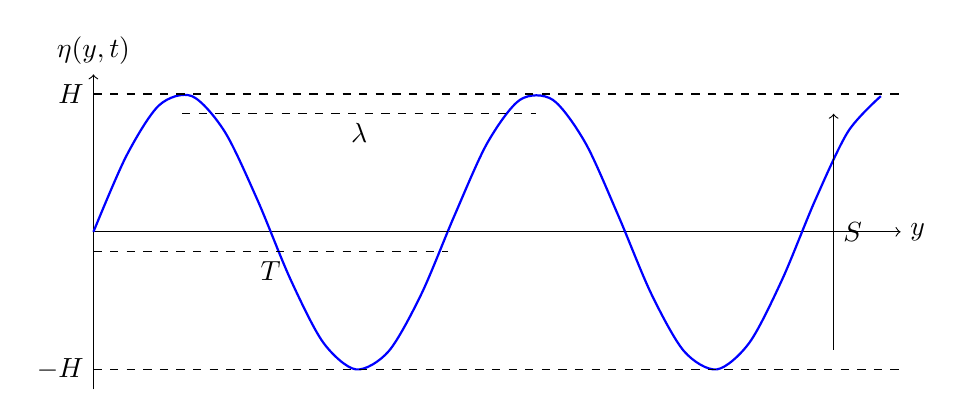
\begin{tikzpicture}[x=0.5cm, y=0.5cm]
    % Draw axes
    \draw[->] (0,-4) -- (0,4) node[above] {$\eta(y,t)$};
    \draw[->] (0,0) -- (20.5,0) node[right] {$y$};
    % Draw wave
    \draw[blue, thick, domain=0:20, smooth] plot (\x, {3.5*sin(2*pi*\x/9 r)});
    % Draw wave height
    \draw[dashed] (0,3.5) node[left] {$H$} -- (20.5,3.5);
    % Draw wave period
    \draw[dashed] (0,-0.5) -- (9,-0.5) node[midway, below] {$T$};
    \draw[dashed] (0,-3.5) node[left] {$-H$} -- (20.5,-3.5);
    % Draw wavelength
    \draw[dashed] (2.25,3) -- (11.25,3) node[midway, below] {$\lambda$};
    \draw[dashed] (5,0) -- (10,0);
    % Draw wave steepness
    \draw[->] (18.8,-3) -- (18.8,3) node[midway,right] {$S$};
\end{tikzpicture}

\end{document}

